\documentclass[compress]{beamer}
%\documentclass[handout]{beamer}

\mode<presentation>
{
  \usetheme{CambridgeUS}      % or try Darmstadt, Madrid, Warsaw, ...
  \usecolortheme{default} % or try albatross, beaver, crane, ...
  \usefonttheme{default}  % or try serif, structurebold, ...
  \setbeamertemplate{navigation symbols}{}
  \mode<beamer>{\setbeamertemplate{blocks}[rounded][shadow=true]}
  \setbeamertemplate{caption}[numbered]
  \useoutertheme{infolines}
  \useoutertheme[subsection=false]{miniframes}
} 

\usepackage[english]{babel}
\usepackage[utf8x]{inputenc}
\usepackage{pifont}
\usepackage{amssymb}
\usepackage{xcolor}
\usepackage{tikz}
\newcommand{\xmark}{\ding{55}}%
\usepackage{eurosym}
\usepackage{graphicx}
\usepackage{comment}
% set colors
\definecolor{myNewColorA}{RGB}{0, 45,114}
\definecolor{myNewColorB}{RGB}{0, 45,114}
\definecolor{myNewColorC}{RGB}{0, 45,114} % {130,138,143}
\setbeamercolor*{palette primary}{bg=myNewColorC}
\setbeamercolor*{palette secondary}{bg=myNewColorB, fg = white}
\setbeamercolor*{palette tertiary}{bg=myNewColorA, fg = white}
\setbeamercolor*{titlelike}{fg=myNewColorA}
\setbeamercolor*{title}{bg=myNewColorA, fg = white}
\setbeamercolor*{item}{fg=myNewColorA}
\setbeamercolor*{caption name}{fg=myNewColorA}
\setbeamercolor{date in head/foot}{fg=white}
\setbeamercolor{page number in head/foot}{fg=white}


\titlegraphic{%
\vspace{0cm}
    
\includegraphics[width=4cm]{logo-vertical2.png}
}

\usepackage{subcaption}
% \usepackage{mathrsfs}

\usepackage{dirtytalk}
\usepackage{tcolorbox}
\usepackage{multicol}
\usepackage{multirow}
\usepackage{caption}
\usepackage{threeparttable}
\usepackage{pdfpages}
\usepackage{longtable}
\usepackage{adjustbox}
\usepackage{colortbl}
\usepackage{tikz}
\def\checkmark{\tikz\fill[scale=0.4](0,.35) -- (.25,0) -- (1,.7) -- (.25,.15) -- cycle;} 
\usepackage{pdfpages}

\usepackage{accents}
\newcommand{\ubar}[1]{\underaccent{\bar}{#1}}
%\usepackage{enumitem}

%% References - BEGIN
\usepackage[backend=bibtex8,style=authoryear-icomp,doi=false,url=false,isbn=false,eprint=false]{biblatex}
\renewbibmacro{in:}{}		% gets rid of the 'In' in front of the journal name
%\bibliographystyle{natbib}        
% \bibliography{references.bib}

% diagram (tree)
\usepackage{tikz}
\tikzset{
  treenode/.style = {shape=rectangle, rounded corners,
                     draw, align=center,
                     top color=white,
                     bottom color=blue!20},
  root/.style     = {treenode, font=\Large,
                     bottom color=red!30},
  env/.style      = {treenode, font=\ttfamily\normalsize},
  dummy/.style    = {circle,draw}
}

% Title page details: 
\title{Chapter 21 \& 13: Consumer theory \& Costs of production} 
\author{Jamie Hyder \\
    Discussion section 4}
\date{October 10, 2025}

\begin{document}

% Title page
\begin{frame}
    \titlepage 
\end{frame}

\begin{frame}{Outline}
    Today we will talk about:
    \begin{itemize}
        \item The theory of the consumer
        \begin{itemize}
            \item budget constraints
            \item indifference curves
        \end{itemize}
        \item Costs of production
    \end{itemize}
\end{frame}

\begin{frame}{Budget constraints}
Most consumers want to increase the quantity/quality of the goods they consume, but money isn't infinite :(

\begin{block}{Consumers face a \textbf{budget constraint:}}
    the limit on the consumption bundles that a consumer can afford
\end{block}
    \vspace{3mm}
\textit{Example: A consumer would like to purchase pasta and wine. They have \$100 to spend, pasta costs \$20 per plate and wine costs \$10 per glass}...
\begin{enumerate}
    \item How much of each good could they consume?
    \item What is the equation for their budget constraint?
    \item What does their budget constraint look like graphically?
    \item What happens if the price of pasta decreases to \$10?
    \item What happens if income increases to \$160?
\end{enumerate}
\end{frame}

\begin{frame}{Representing preferences}
\begin{center}
    How do we know which bundle of goods a consumer prefers?
\end{center}
    \begin{block}{We can represent preferences using \textbf{indifference curves:}}
IC: a curve showing consumption bundles that give the consumer \textit{equal levels of satisfaction}

\vspace{3mm}

The slope at any point on an indifference curve equals the \textbf{Marginal Rate of Substitution (MRS)}: the rate at which a consumer is willing to give up one unit of good X for another unit of good Y
    \end{block}

    \vspace{2mm}

    We calculate MRS as follows:
    \[MRS = \frac{MU_X}{MU_Y}\]
\end{frame}

\begin{frame}{Properties of indifference curves:}
    \begin{enumerate}
        \item Higher indifference curves are preferred to lower ones: 
        \begin{enumerate}
            \item More is better!
        \end{enumerate}
        \item Indifference curves are downward sloping: 
        \begin{enumerate}
            \item in most cases a consumer likes both goods, so to decrease plates of pasta but keep the same satisfaction, we must increase glasses of wine
        \end{enumerate}
    \item Indifference curves do not cross
    \begin{enumerate}
        \item If they crossed, we would violate the assumption that people prefer more to less
    \end{enumerate}
    \item Indifference curves are bowed inwards
    \begin{enumerate}
        \item MRS is not constant... we are more willing to give up a good we already have an abundance of
    \end{enumerate}
    \end{enumerate}
\end{frame}

\begin{frame}{Optimizing}
A consumer wants to maximize their satisfaction given their budget constraint... 

\begin{block}{This is achieved by choosing the bundle where either:}
    \begin{itemize}
        \item Their indifference curve is tangent to their budget constraint (where they touch... kind of)
        \item The MRS is equal to the slope of the budget constraint
    \end{itemize}
\end{block}

When income or prices of goods change, our budget constraint does too, and so we would find ourselves on a new indifference curve at optimum... 
\end{frame}

\begin{frame}{Income \& Substitution Effects}
    When the price of goods changes, the resulting change to the budget constraint and optimal bundle is a result of two effects:
    \begin{enumerate}
        \item \textbf{Income effect:} Change in consumption that results when a price change \textit{moves the consumer to a higher or lower indifference curve}
        \item \textbf{Substitution effect:} Change in consumption that results when a price change \textit{moves the consumer along a given indifference curve to a point with a new MRS}
    \end{enumerate}

    \vspace{4mm}

\begin{center}
    ** A change in income results only in an income effect **
    \end{center}
\end{frame}

\begin{frame}{Costs of Production}
    A firm aims to maximize their profit:
    \[\text{Profit} = \text{total revenue} - \text{total cost}\]
\begin{itemize}
    \item total revenue: \(TR = P \times Q\)
    \item total cost is the sum of all \textbf{implicit} and \textbf{explicit} costs of inputs to production
    \begin{itemize}
        \item \textbf{Implicit}: input costs which \textit{do not} require monetary outlay from the firm
        \item  \textbf{Explicit}: input costs which \textit{do} require a monetary outlay from the firm
    \end{itemize}
\end{itemize}
\end{frame}

\begin{frame}{Types of Profit}
    There are two types of profit we can consider:
    \begin{block}{Economic Profit:}
        total revenue less implicit \textit{and} explicit costs
    \end{block}

    \begin{block}{Accounting}
        total revenue less explicit costs \textit{only}
    \end{block}
\end{frame}

\begin{frame}{Costs}
\begin{block}{Types of costs:}
    \begin{itemize}
    \item Fixed costs: costs that do not vary with Q
    \item Variable costs: costs that vary with Q
\end{itemize}
\end{block}

\begin{block}{Measures of costs:}
\begin{itemize}
    \item Average total cost (ATC): \(ATC = TC/Q\)
    \item Average fixed cost (AFC): \(AFC = FC/Q\)
    \item Average variable cost (AVC): \(AVC = VC/Q\)
    \item Marginal Cost: \(MC = \Delta TC/\Delta Q\)
\end{itemize}
\end{block}
\end{frame}

\begin{frame}{Example}
    Consider a firm which produces pizzas:
    
    \vspace{3mm}
    
     A worker costs \$100 and the firm has fixed costs of \$200. 
     
     \vspace{3mm}
     
         The following table shows the number of pizzas produced given varying numbers of workers. Let's add information for the marginal product, total cost, average total cost, and marginal cost.
    \begin{table}[H]
        \centering
        \begin{tabular}{cc}
            Workers & Output \\
            \hline
            0 & 0 \\
            1 & 20 \\
            2 & 45 \\
            3 & 80 \\
            4 & 100 \\
            5 & 110 \\
        \end{tabular}

        \label{tab:placeholder}
    \end{table}
\end{frame}

\begin{frame}{What do costs look like?}
\begin{figure}
        \centering
        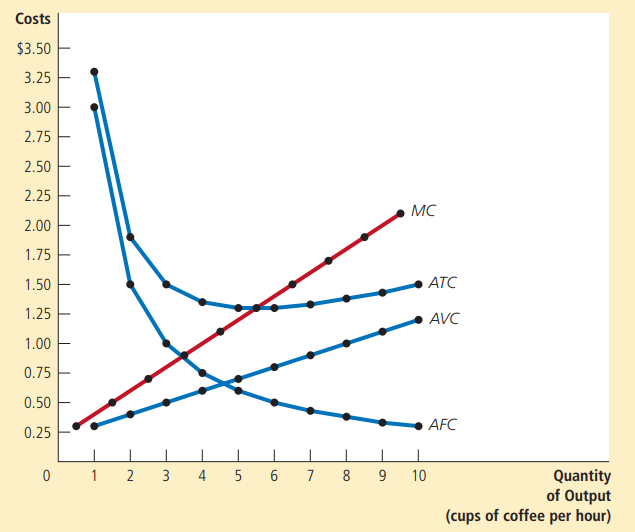
\includegraphics[width=0.65\linewidth]{uTC.png}
        \caption{Relationship between costs}
        \label{fig:placeholder}
    \end{figure}
\end{frame}

\begin{comment}
\begin{frame}{Economies and Diseconomies of Scale}
    We can define the scale of production in the following 3 ways:
    \begin{enumerate}
        \item Economies of Scale: Long run ATC declines as Q increases
        \item Diseconomies of Scale: Long run ATC increases as Q increases
        \item Constant returns to scale: Long run ATC stays the same as Q changes
    \end{enumerate}
\end{frame}
\end{comment}


\end{document}